\section{Experiment 2}
\label{Exp2}
\setlength{\parindent}{20pt}
\justifying

\subsection{Methods}
\label{Methods2}

\subsubsection{\large{\emph{Participants}}}
\label{Participants2}

\noindent
All participant criteria were identical to experiment 1.

\subsubsection{\large{\emph{Stimuli}}}
\label{Stimuli2}

\noindent
All stimuli parameters were identical to experiment 1.

\subsubsection{\large{\emph{Procedure}}}
\label{Procedure2}
\noindent \underline{Morpheme spelling task}

\noindent
Given that the current task requires initial segmentation and subsequent co-occurrence tracking, and that the latter is the process we were most interested in, a new task was devised with the aim of facilitating segmentation. This would allow participants to spend fewer cognitive resources on this step, hopefully allowing for better co-occurrence tracking. Therefore, a familiarisation task with all the morphemes presented in training was given as the first task in the experiment.

\begin{figure}[!htbp]
    \begin{center}
        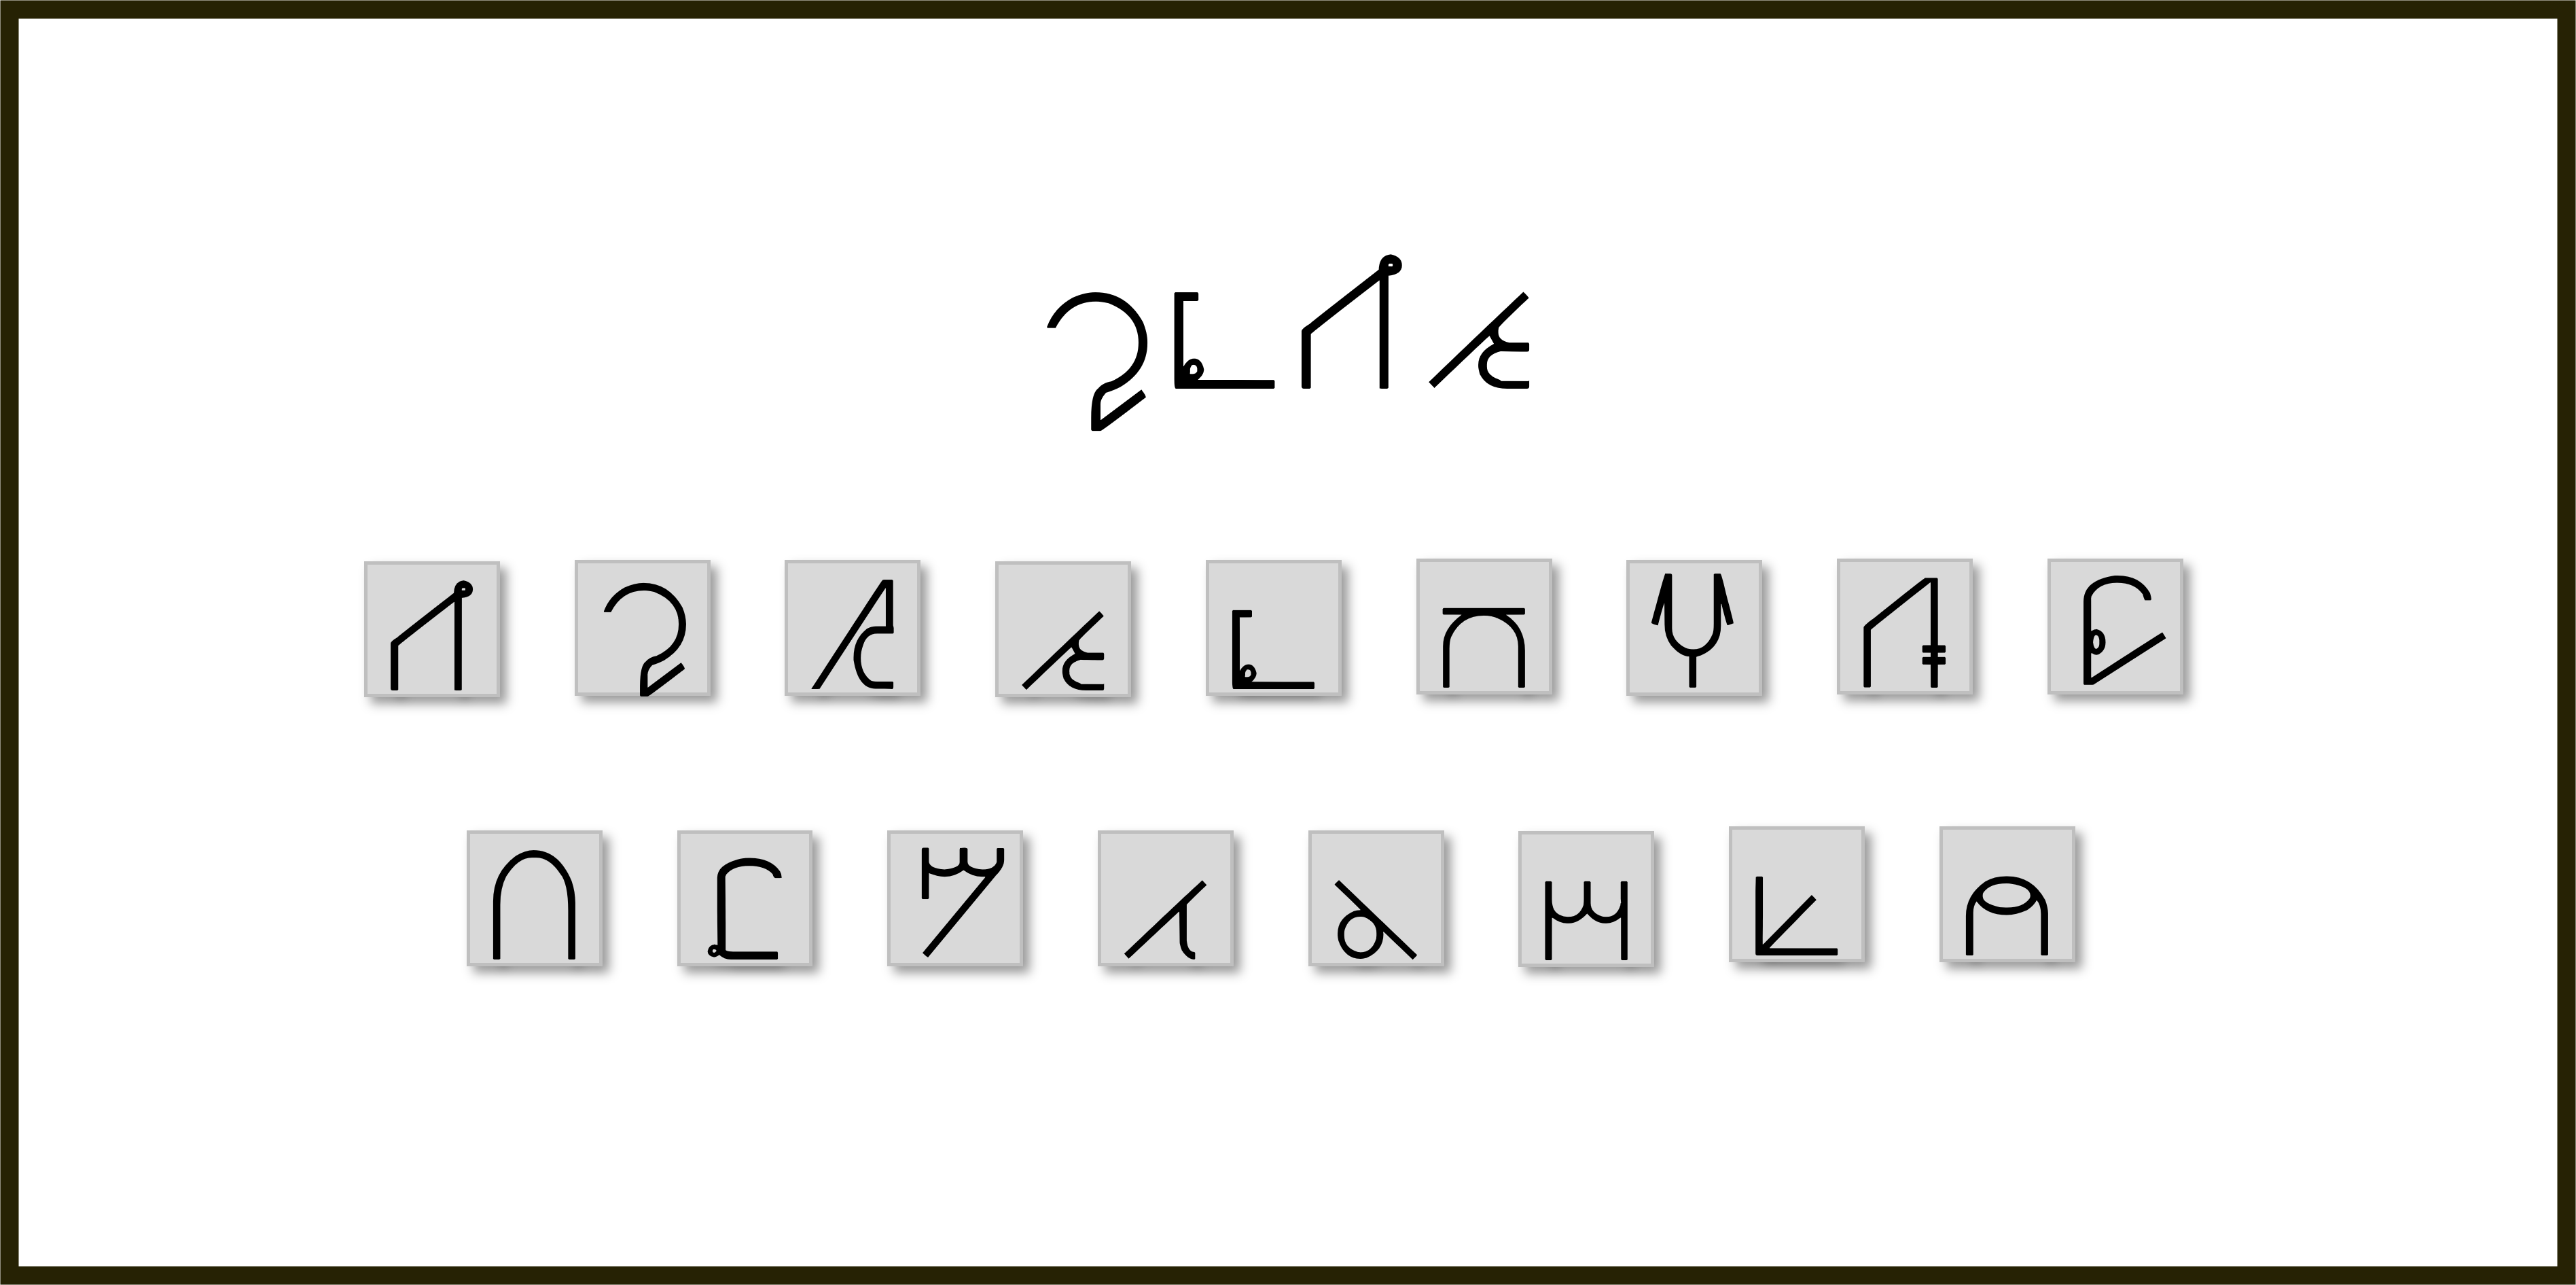
\includegraphics[width=0.6\textwidth]{Figures/MorphemeSpellingExample.png}
    \end{center}
    \caption[]{\justifying Example item of the morpheme spelling task. A target morpheme is shown above with all of the individual letters used in the experiment in a keyboard below. A participant must click each letter to form the target morpheme.}
    \label{morph_spelling}
\end{figure}

In order to ensure that participants were actively learning the morphemes rather than being passively exposed to them, a spelling task was created (illustrated in \autoref{morph_spelling}). This procedure would also help participants get used to the unfamiliar BACS-1 characters. Participants were presented with each morpheme that was to be used in the experiment, and had to click on each composing letter on the on-screen BACS-1 keyboard. Each morpheme was displayed until the participant completed its spelling. We introduced each of the 30 morphemes once. 


\noindent \underline{Training}

\noindent
The aforementioned coding error was resolved, presenting participants 8 true training blocks.


\subsubsection{\large{\emph{Analysis}}}
\label{Analysis2}

\noindent
This time, the analysis included all items in each of the testing conditions, and all morphemes in the familiarity test. All data was analysed in precisely the same way as in experiment 1.